\chapter{Gestión del proyecto}\label{ch:gestion}

\section{Alcance}\label{sec:alcance}

El alcance de este proyecto incluye el trabajo necesario para diseñar,
implementar y documentar un framework de modelado y desarrollo de simulación de
sistemas dinámicos discretos basados en eventos. Dicho framework se dividirá en
tres módulos principales:
\begin{itemize}
    \item \textbf{Lenguaje}: Un lenguaje de modelado específico pensado para ser usado
    por usuarios que no tengan mucha experiencia en programación. Se hará uso de
    las herramientas de desarrollo de compiladores Flex y Bison para generar un
    transpilador que traduzca ficheros de este lenguaje a código Python. A
    través de él se plantea:
    \begin{itemize}
        \item Permitir la rápida implementación de este tipo de modelos a través
        de grafos de sucesos.
        \item Permitir que el programador del lenguaje se encargue sólo de
        realizar las implementaciones pertinentes al sistema de simulación que
        desee desarrollar:
        \begin{itemize}
            \item Especificación de las variables globales, variables de
            entrada, contadores estadísticos y medidas de rendimiento propias
            del modelo.
            \item Inclusión de eventos adicionales y sus acciones
            correspondientes.
            \item Creación y eliminación de eventos en función de tiempo y
            condiciones lógicas.
            \item Inclusión de código adicional escrito directamente en Python
            en caso de ser necesario.\urgent{Cambiar redacción}
        \end{itemize}
    \end{itemize}
    \item \textbf{Núcleo}: Una serie de módulos que implementarán un microframework de
    simulación de este tipo de sistemas en específico para Python, pensado para
    ser usado por programadores y para acotar la traducción del nuevo lenguaje.
    A través de él se plantea:
    \begin{itemize}
        \item Permitir que la traducción del lenguaje incluya dentro del fichero
        generado las estructuras de datos, funciones y procedimientos que tienen
        en común todos los sistemas dinámicos discretos: \urgent{Aquí te falta
        la posibilidad de poner las cosas variables también}
        \begin{itemize}
            \item Generadores de datos aleatorios para distintos tipos de
            distribuciones.
            \item Reloj y temporizador de simulación para ejecutar los eventos.
            \item Estructura de datos para almacenar los sucesos según deben
            ocurrir en el tiempo.
            \item Las respectivas implementaciones mínimas de los dos eventos
            que siempre formarán parte de todos los modelos: “Inicio” y “Fin”.
            \item Generador de informes final que se ejecutará al finalizar la
            simulación y mostrará los resultados que se deseaban estudiar con
            ésta.
        \end{itemize}
    \end{itemize}
    \item \textbf{CLI}: Una interfaz de comandos por terminal que se usará para
    gestionar, configurar y ejecutar los proyectos desarrollados con este
    framework.
\end{itemize}


% -----------------------------------------------------------------------------


\subsection{Objetivos}\label{subsec:objetivos}

\subsubsection{Objetivo general}
Generar un lenguaje de modelado de simulación de sistemas dinámicos discretos
basados en eventos junto con un transpilador que lo traduzca a Python, un
microframework para acotar la traducción y un CLI para gestionar proyectos
desarrollados con este producto.

\subsubsection{Objetivos específicos}
\begin{enumerate}
    \item Diseñar un nuevo lenguaje de modelado y simulación de sistemas
    dinámicos discretos basados en eventos usando las herramientas de desarrollo
    de procesadores de lenguaje Flex y Bison.
    \item Diseñar, implementar y verificar una serie de módulos y
    funcionalidades realizadas en Python con el fin de generar un microframework
    para simular estos mismos sistemas.
    \item Implementar y verificar un transpilador que traduzca el lenguaje del
    producto a Python usando las características del objetivo anterior.
    \item Diseñar, implementar y verificar una serie de operaciones accesibles
    desde una CLI de cara a ser usadas para la gestión, configuración y
    ejecución parametrizada de simulaciones realizadas con el producto.
    \item Implementar distintas técnicas de análisis de salidas, experimentación
    y optimización de modelos dentro del núcleo del framework.
    \item Desarrollar un manual de usuario que contendrá toda la documentación
    necesaria para hacer uso del framework.
\end{enumerate}


% -----------------------------------------------------------------------------


\subsection{Requisitos}\label{subsec:requisitos}
El requisito base principal del proyecto consiste en cumplir con un tiempo de
dedicación total máximo de 300 horas.
% Sin embargo, se pueden listar otros requisitos específicos:

% \subsubsection{Caracterización de la memoria}
% \begin{itemize}
%     \item Debe ser bien citado y referenciado.
%     \item Apartado de calidad.
% \end{itemize}

% \subsubsection{Caracterización del framework}
% \begin{itemize}
%     \item Un lenguaje verificado que no pete a la primera
%     \item El resultado son métricas en un dataframe (o varios si harás lo de
%     validación)
%     \item Cumplir con la línea base de calidad definida en el apartado (...)
% \end{itemize}

% \subsubsection{Caracterización del manual}
% \begin{itemize}
%     \item Utilizar referencias a recursos ajenas
% \end{itemize}

% \subsubsection{Licencia del producto}


% -----------------------------------------------------------------------------


% \subsection{Entregables}

% \begin{itemize}
%     \item Memoria: \change{Relacionados con el objeto de proyecto en sí}
%     \item Framework: \change{Relacionados con el objeto de proyecto en sí}
%     \item Manual: \change{Relacionados con el objeto de proyecto en sí}
% \end{itemize}


% -----------------------------------------------------------------------------


% \subsection{Exclusiones}

% Mi proyecto devolverá los datos en un sólo formato, no devolveré más tipos de
% ficheros para darle gusto al usuario.


% -----------------------------------------------------------------------------


% \subsection{Supuestos}

% \urgent[inline]{}


% -----------------------------------------------------------------------------


\subsection{EDT}\label{subsec:edt}

\begin{figure}[H]
    \centering
    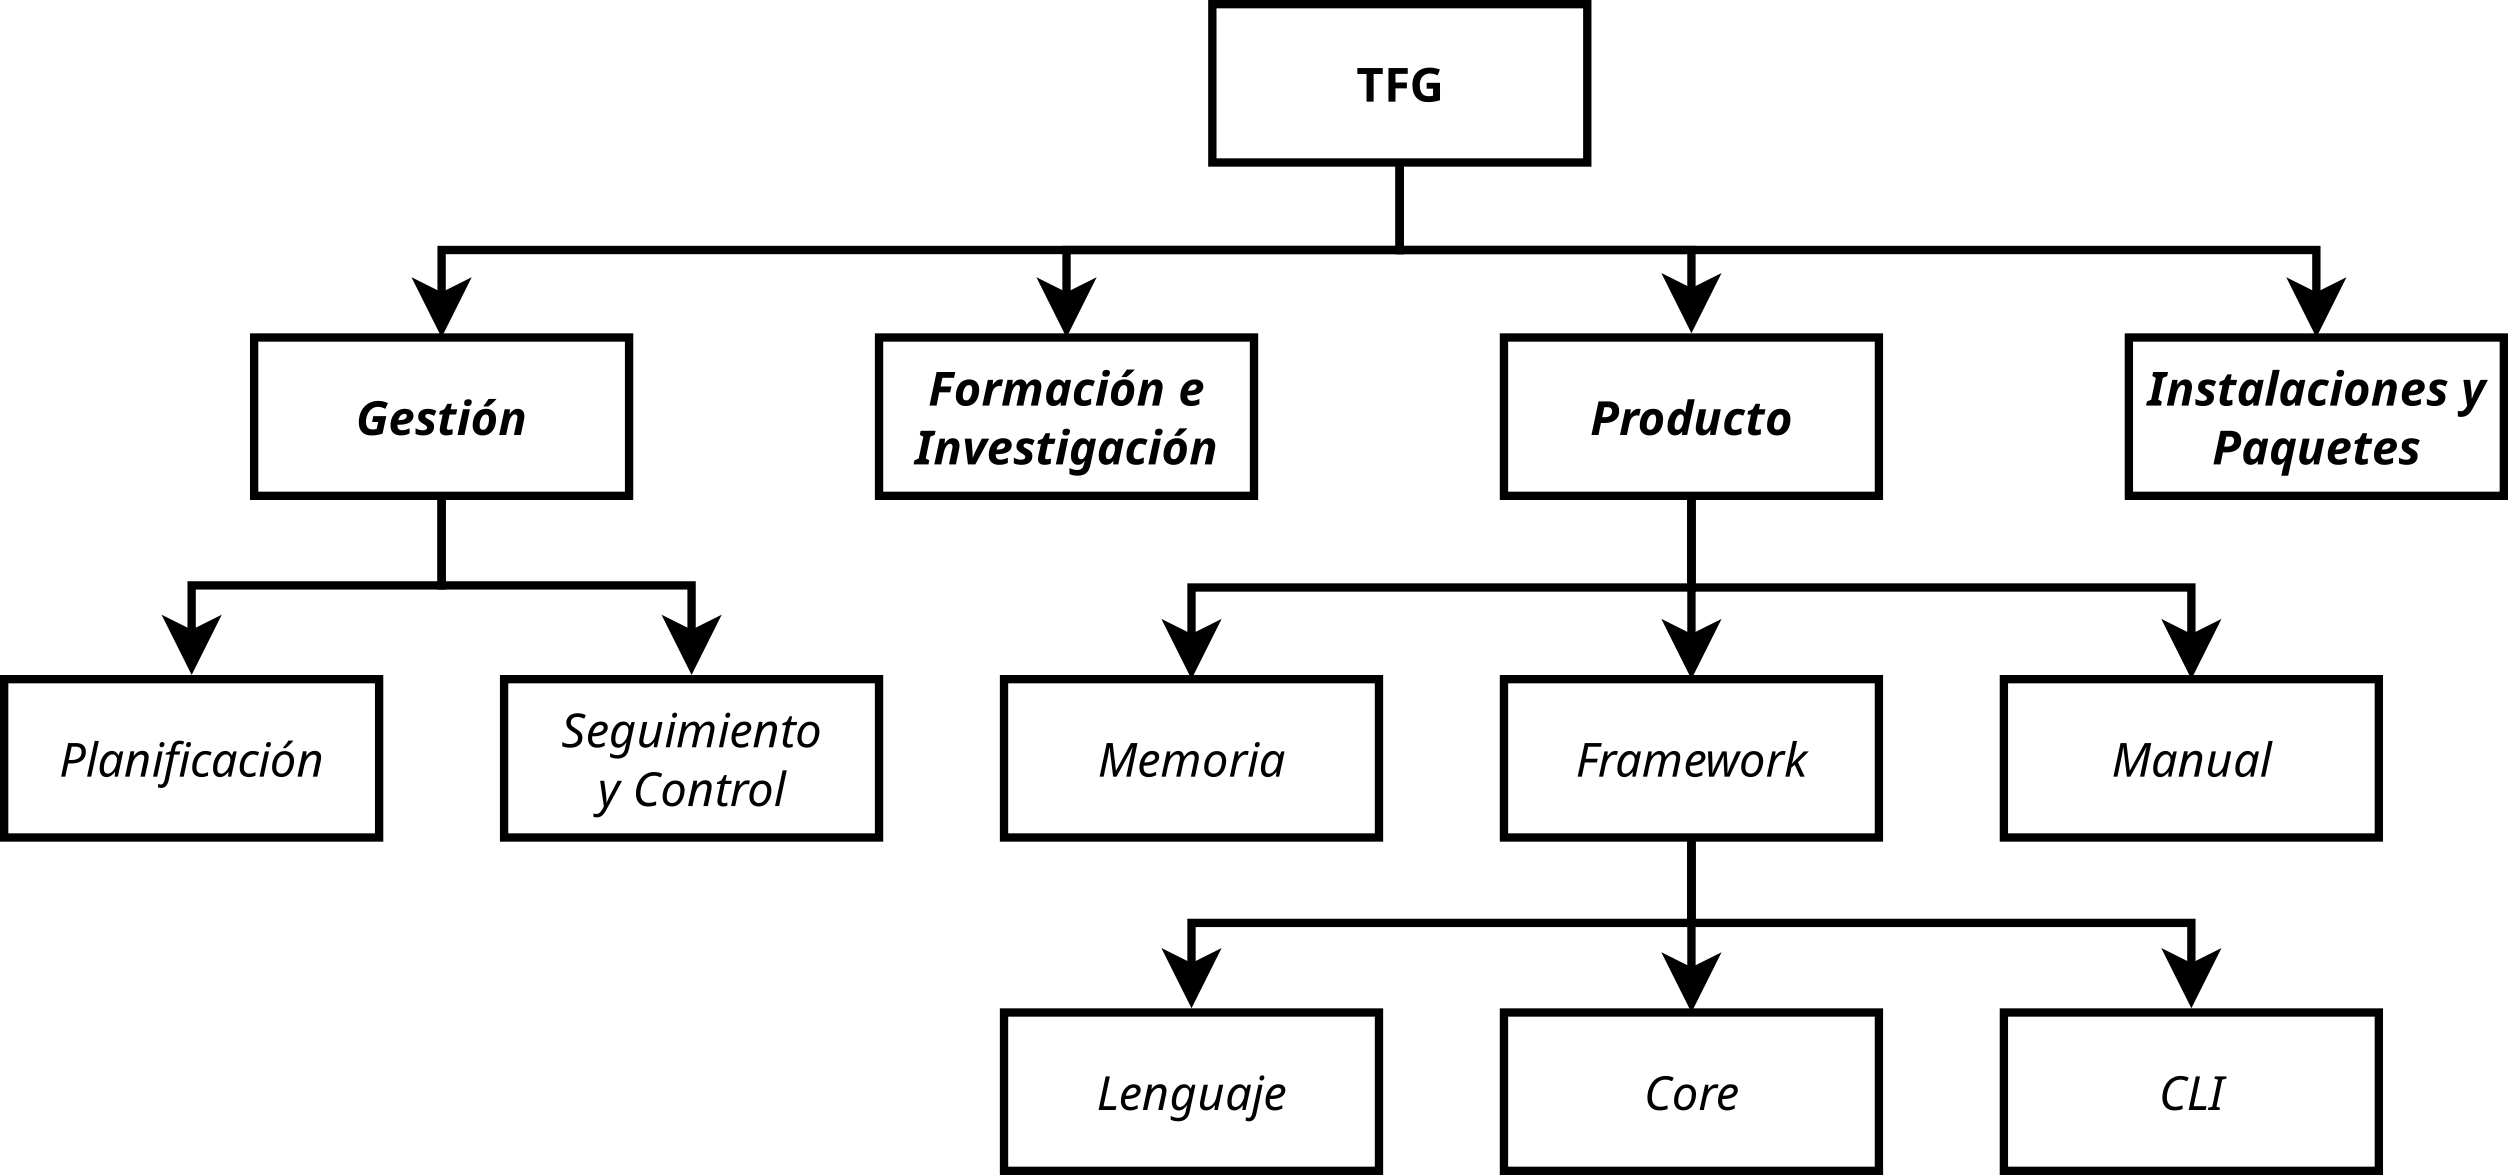
\includegraphics[width=0.8\textwidth]{5-Cuerpo/Chapter1/EDT.png}
    \caption{Esquema de Descomposición de Trabajo del Proyecto}
    \label{fig:EDT}
\end{figure}

\subsubsection{Rama de Gestión}
El paquete de trabajo \textbf{Gestión (Ge)} contendrá:
\begin{itemize}
    \item \textbf{Planificación (Ge.P):} Este paquete de trabajo agrupará todas
    las tareas relacionadas a la realización de la planificación y preparación
    inicial del proyecto.
    \item \textbf{Seguimiento y Control (Ge.S):} Este paquete de trabaj agrupará
    todas las tareas necesarias para asegurar que el seguimiento del proyecto
    está realizando como se plantea en la planificación y, en caso de no ser
    así, controlar las consecuencias de las desviaciones emergentes.
\end{itemize}

\subsubsection{Rama de Formación e Investigación}
El paquete de trabajo \textbf{Formación e Investigación (FeI)} contendrá todas
las tareas relacionadas con el aprendizaje de herramientas, búsqueda de
referencias y recolección de información necesaria para el desarrollo del
proyecto.

\subsubsection{Rama de Producto (Pr)}
El paquete de trabajo \textbf{Producto (Pr)} contendrá todas las tareas
relacionadas al propio diseño, implementación y verificación de los entregables
principales del proyecto. Podemos desglosarlo en tres paquetes más pequeños:
\begin{itemize}
    \item \textbf{Memoria (Pr.Me):} Este paquete de trabajo agrupará todas las
    tareas necesarias para la realización de la memoria final del proyecto.
    \item \textbf{Framework (Pr.Fr):} Este paquete de trabajo agrupará todas las
    tareas relacionadas al desarrollo del framework planteado en el alcance del
    proyecto. Podemos separarlo en sus tres partes principales:
    \begin{itemize}
        \item \textbf{Lenguaje (Pr.Fr.Le):} Este paquete contendrá todas las
        tareas relacionadas al diseño y desarrollo del nuevo lenguaje de
        modelado.
        \item \textbf{Core (Pr.Fr.Co):} Este paquete contendrá todas las
        tareas relacionadas al diseño y desarrollo del propio núcleo del
        framework.
        \item \textbf{CLI (Pr.Fr.Cli):} Este paquete contendrá todas las
        tareas relacionadas al diseño y desarrollo de la interfaz de comandos
        proporcionada para facilitar la gestión de proyectos realizados con el
        a generar.
    \end{itemize}
    \item \textbf{Manual (Pr.Ma):} Este paquete de trabajo agrupará todas las
    tareas necesarias para la realización del manual de usuario que se generará
    para facilitar el uso del producto a desarrollar.
\end{itemize}

\subsubsection{Rama de Instalación y Paquetes}
El paquete de trabajo \textbf{Instalación y Paquetes (IyP)} agrupará todas las
tareas relacionadas a la preparación del entorno de desarrollo y la instalación
de paquetes y dependencias para la realización del producto principal del
proyecto.

% \subsubsection{Rama de Defensa (De)}
\section{Metodología}\label{sec:metodologia}

A la hora de gestionar un proyecto, es recomendable definir una metodología de
trabajo, seguimiento y control con el fin de asegurar el correcto cumplimiento y
finalización de su lista de requisitos y objetivos. Tras investigar y plantear
distintas alternativas, se ha escogido la metodología Kanban para desarrollar
este proyecto.

El método Kanban como tal es útil si se desea:
\begin{itemize}
    \item Iniciar un proyecto de manera ágil, rápida, de coste nulo y bajo riesgo. % Getting off to a low-risk, zero-cost, agile, fast start.
    \item Analizar y mejorar el proceso de trabajo ya existente. % Pinning down existing workflows and spotting glaring errors.
    \item Controlar múltiples grupos de tareas. % Controlling multiple pieces of unconnected work.
    \item Asegurar que el número de tareas en ejecución están dentro de un nivel aceptable. % Keeping the numbers of jobs in play down to an acceptable level.
    \item Cambiar a una mentalidad de desarrollo ágil. % Getting the team into an agile way of thinking.
\end{itemize}

Esta sección, por tanto, estará dedicada a explicar los conceptos e ideas
necesarias de cara a justificar la razón por la cual se ha escogido este método
de trabajo. Además, es necesario mencionar que esta información será resumida
principalmente de \cite{Cole2015-fd} y \cite{Stellman2014-qr}, siendo éstas las
referencias recomendadas en caso de desear más detalles al respecto.
\subsection{Definición}

El método Kanban tiene sus orígenes en las fábricas de coches de Toyota a manos
de Taiichi Ohno. Fue creado como un simple sistema de planificación y
administración de trabajo e inventario de cada fase de producción. Sin embargo,
fue David J. Anderson quien definió y adaptó esta metodología para el uso en
ingeniería y desarrollo de software.

Es necesario mencionar que, contrario a lo que se piensa normalmente, Kanban es
una metodología ágil de mejora de procesos y no un framework de administración
de proyectos. Y así como muchos métodos de este tipo, se caracteriza
principalmente por ser evolutivo e iterativo en el tiempo.

Asimismo, Kanban comparte la misma ideología de trabajo con el método Lean hasta
tal punto que se considera que es una especialización de esta última. Aplicando
los principios y valores de este proceso, Kanban se centra en eliminar los
desperdicios de tiempo y recursos que el equipo tiene. Por lo tanto, este
proceso de mejora pide a los equipos de desarrollo empezar con una metodología
ya existente para poder perfeccionarla gradualmente en el tiempo a través de la
experimentación, el cálculo de distintas métricas de rendimiendo y la
confirmación de resultados positivos según dichas medidas.

Todo equipo cuenta con un sistema para la implementación de código, ya sea que
se siga una metodología formal como Scrum o que se disponga de una serie de
reglas no definidas o reconocidas explícitamente. Como consecuencia de esto, lo
único que se necesita para empezar a utilizar Kanban es identificar el proceso
de desarrollo actual para poder formalizarlo y adaptarlo a esta metodología.

Así pues, aunque Kanban no es un sistema de gestión de proyectos, es posible
hacer uso de éste para ello al tener como principal objetivo aumentar la
predictabilidad del flujo de trabajo y así mejorar la planificación del proyecto
como tal.

\subsection{Principios de Kanban}
Al ser una especialización del método Lean, se tiene una serie de principios
directores en esta metodología. Especificamente se pueden listar los siguientes
tres:
\begin{itemize}
    \item \textbf{Empieza con lo que se hace actualmente}: %Start with what you do now
    Como se había mencionado anteriormente, el método Kanban pide requiere de un
    proceso o metodología inicial. Es a través del análisis y la comprensión de
    dicho proceso que Kanban permite perfeccionarlo iterativamente. Pero como
    consecuencia de esto, no es posible aplicar Kanban adecuadamente si se
    desconoce la metodología que usa el equipo de desarrollo.

    \item \textbf{Comprométete al cambio evolutivo e incremental}: %Agree to pursue incremental, evolutionary change
    This is the system that Kanban starts with. The team already has a way to run their
project. Kanban just asks them to understand that system. That's what it means to
start with what you do now. The goal of Kanban is to make small improvements to
that system. That's what it means to pursue incremental, evolutionary change—and
why Kanban has the practice improve collaboratively, evolve experimentally. In
lean thinking, part of seeing the whole is taking measurements, and measurements
are at the core of experimentation and the scientific method. A Kanban team will
start with their system for building software, and take measurements to get an
objective understanding of it. Then they'll make specific changes as a
team—later in this
chapter, you'll learn exactly how those changes work—and check their measurements
to see if those changes have the desired effect.
    \item \textbf{Respeta el proceso, los roles, las responsabilidades y títulos actuales}: %Respect the current process, roles, responsibilities and titles
    The Lean value of amplifying learning is also an important part of evolving the system that your team uses to build software. Throughout this book you've learned
about feedback loops. When you collaborate to measure the system and evolve
experimentally, those feedback loops become a very important tool for gathering
information and feeding it back into the system; the Kanban practice of
implementing feedback loops should make sense to you, and should help you to see
how Kanban and Lean are closely linked.
Amplifying learning also factors into the Kanban principle of initially
respecting current roles and responsibilities. For example, say that a team
always starts each project
with a meeting between a project manager, a business analyst, and a programmer.
They may not have written down a rule for what goes on in that meeting, but you
probably have a good idea of what goes on in it just from reading those job titles.
That's one reason why Kanban respects current roles, responsibilities, and job titles—
because they're an important part of the system.
A common theme between all of these principles is that Kanban only works for a
team when they take the time to understand their own system for building software.
If there was one right way to build software, everyone would just use it. But we
started this book by saying back in Chapter 2 that there is no silver bullet—there's no
single set of “best” practices that will guarantee that a team builds software right every
time. Even the same team, using the same practices, can have success with one project
but fail miserably in the next one. This is why Kanban starts with understanding the
current system for running the project: once you see the whole system, Kanban gives
you practices to improve it.
\end{itemize}

\subsection{Prácticas de Kanban}

El método Kanban, además, define explícitamente una serie de prácticas a llevar
a cabo con el fin de aplicar correctamente la mejora de procesos que éste
permite. Sin embargo, no es totalmente necesario hacer uso de todas estas en su
totalidad al iniciar con el método. El método tiene específicamente los
siguientes seis principios:

\begin{itemize}
    \item \textbf{Definir y visualizar el flujo de trabajo}: %Define and Visualise Workflow
    Kick off with a visual representation of the flow of work going from to-do to
    done status. Many prefer to add only one other step in between: in progress.
    Others prefer to break the workflow down into a series of procedural stages such
    as: plan, design, draft, build, test, deploy, with to-do and done as bookends.
    In Kanban, visualizing means writing down exactly what the team does, warts and
    all, without embellishing it. This is part of lean thinking: a Kanban team takes
    the Lean principle of see the whole very seriously. When the team has the right
    mindset, it just feels wrong to tinker with the workflow while you're trying to
    visualize it, because that would interfere with seeing the whole. The value of
    decide as late as possible is also important here: you don't have all of the
    information about how you build software yet, so there's a later responsible
    moment to make decisions about how you'll change it. A kanban board is a tool
    that teams use to visualize their workflow. (The K in the methodology name
    Kanban is typically uppercase; the k in kanban board is usually lowercase.)

    \item \textbf{Limitar el trabajo en progreso}: %Limit work-in-progress
    Trying to do too many things at
    the same time is a proven recipe for disaster; it applies equally
    at an individual level and to teams. Kanban limits the number
    of items allowed to be on the go at any one time - known as
    the work-in-progress (WiP) - to ensure optimum efficiency.
    Common sense is enough to get started and then experience
    will help fine tune to pin down the optimal WiP limit.
    A team can only do so much work at a time. We learned this with both Scrum and
    XP, and it's an important part of lean thinking as well. When a team agrees to do
    more work than they can actually accomplish by the time they'd agreed to deliver it,
    bad things happen. They either leave some of the work out of the delivery, do a poor
    job of building the product, or work at an unsustainable pace that will cost dearly in
    future releases. And sometimes it's not obvious that a team has taken on more work
    than they can handle: each individual deadline may seem reasonable for the work
    being done, but if each person is expected to multitask on multiple projects or tasks at
    the same time, the team slowly becomes overburdened, and the extra effort required
    for task switching can eat up as much as half of their productivity.
    Visualizing the workflow helps the team see this overburdening problem clearly, and
    that's the first step toward fixing the problem. Unevenness and overburdening—
    which we learned about in Chatper 8—become clear on the kanban board when
    stickies always pile up in one column. Luckily, queuing theory doesn't just alert us to
    the problem; it also gives us a way to fix it. Once unevenness in the workflow has
    been identified, we can use it to control the amount of work that flows through the
    whole system by placing a strict limit on the amount of work that is allowed to pile up
    behind it. This is what's behind the Kanban practice limit work in progress.
    Limiting work in progress (WIP) means setting a limit on the number of work items
    that can be in a particular stage in the project's workflow. A lot of people tend to focus
    on moving work items through the workflow as fast as they can. And for a single
    work item, that workflow is linear: if you're a developer and you're done with the
    design for a feature, and your workflow says that the next thing you do with it is build
    it and then send it on to a tester, the next thing you're going to do is build the code
    for it—and it's easy to become fixated on getting that feature built and sent on to the
    tester as quickly as possible because it was the last thing you were working on.
    But what if the test team is already working on more features than they can test right
    now? It doesn't make sense to jump into development for this feature if it will just end
    up waiting around because nobody's ready to test it. That would cause overburdening
    for the test team. So what can be done about it?
    For this, Kanban goes back to lean thinking—specifically, the principle of options
    thinking that you learned about in Chapter 8. One reason that a Kanban team uses a
    kanban board is because it shows all of your options. If you're that developer who just
    finished the design for a feature, it's easy to think that you now have a commitment to
    work on the code next. But working on the code for that particular feature is an
    option, not a commitment. When you look at the whole kanban board, you'll see
    many stickies that you can work on next. Maybe there are other stickies in earlier col-
    umns for other features that need to be designed, or ones in later columns for features
    with bugs that the testers found that need to be fixed. In fact, most of the time you
    have many options that you can choose from. Which do you choose first?
    Setting a WIP limit for a step in your workflow means limiting the number of fea-
    tures that are allowed to move into that step. This helps limit the team's options to
    make that decision easier in a way that will prevent overburdening and keep the fea-
    tures flowing through the workflow as efficiently as possible. When you finish
    designing that feature, for example, and you see that the workflow is already at its
    limit for writing code, then you'll look for other options and work on them instead—
    and the test team won't get overburdened. (Think about this for a minute: can you see
    how this will reduce the average lead time for a feature? If so, then you're starting to
    get the hang of systems thinking!)

    \item \textbf{Manejar el flujo de trabajo}: %Manage the flow of work
    The aim is to achieve a fast,
    smooth movement from to-do to done. If so it means the
    process is operating at optimum efficiency thus creating
    maximum business value in the shortest time possible. An
    important add-on is for it to be repeatable and consistent.
    As teams continue to deliver work, they identify workflow problems and adjust their
WIP limits so that the feedback loops provide enough information without causing
thrashing. The flow of the system is the rate at which work items move through it.
When the team finds an optimal pace for delivery combined with a comfortable
amount of feedback, they've maximized the flow. Cutting down on the unevenness
and overburdening, and letting your teams finish each task and move on to the next
one, increases the flow of work through your project. When unevenness in the system
causes work to pile up, it interrupts the work and decreases the flow. A Kanban team
uses the manage flow practice by measuring the flow and taking active steps to
improve it for the team.
You already know what it feels like when work is flowing. You feel like you're getting a
    lot accomplished, and that you aren't wasting time or stuck waiting for
    someone else to do something for you. The personal feeling of being on a team with a lot of flow is
    that every day, all day, you have the feeling that you're doing something valuable.
    That's what everyone is striving for.
    You also know what it feels like when work doesn't flow. It feels like you're mired in
    muck, and that you're barely making progress. It feels like you're always waiting for
    someone to finish building something that you need, or to make a decision that
    affects your work, or to approve some ticket, or somehow always find some other way
    to block your work—even when you know that nobody is intentionally trying to
    block it. It feels uncoordinated and disjointed, and you spend a lot of time explaining
    to other people why you're waiting. It's not that you're underallocated; your project
    team is probably 100\% allocated, or even overallocated. But while your project plan
    may say that you're 90\% done, it feels like there's still 90\% of the project left to go.
    And your users know what it feels like when work doesn't flow, because their lead
    times keep going up. It seems like the team takes longer and longer to respond to
    their requests, and even simple features seem to take forever to build.
    The whole point of Kanban is to increase flow, and to get the whole team involved in
    increasing that flow. When the flow increases, frustration with unevenness and long
    lead times decreases.

    \item \textbf{Hacer explícitas las políticas de proceso}: %Make the process explicit
    An unambiguous statement
    of how work gets done is essential for any objective review.
    With a common understanding it's easier to discuss issues
    impartially and reach a consensus on improvements. There
    must be a natural checkpoint at the end of each step with
    clear rules for moving on to the next one.

    \item \textbf{Implementar ciclos de retroalimentación}: %Implement Feedback Loops

    \item \textbf{Mejorar colaborativamente}: %Improve collaboratively
    Once the spotlight is on the
    workflow, ideas start to develop about how it can be
    improved. The WiP limit plays a key role in sparking
    discussions by forcing the team to focus on blockers to work
    in play when the limit is reached. An initial cap of no more
    than two tasks per person soon highlights problems that
    impede the flow; then the team simply faces up to those
    issues and resolves them.
\end{itemize}

\subsection{Métricas de flujo}
\urgent{TRADUCIR Y FINALIZAR}
% Orderly Disruption Limited, Daniel S. Vacanti, Inc. Offered for license under the Attribution
% ShareAlike license of Creative Commons, accessible at http://creativecommons.org/licenses/by-
% sa/4.0/legalcode and also described in summary form at http://creativecommons.org/licenses/by-sa/4.0/,
% By using this Kanban GuideTM, you acknowledge that you have read and agree to be bound by the terms of
% the Attribution ShareAlike license of Creative Commons.

\begin{itemize}
    \item \textbf{Trabajo en progreso}: The number of work items started but not finished
    (according to the DoW).
    \item \textbf{Rendimiento}: The number of work items finished per unit of
    time. Note the measurement of throughput is the exact count of work items.
    \item \textbf{Edad del elemento de trabajo}: The amount of elapsed time between when a work
    item started and the current time.
    \item \textbf{Tiempo de ciclo}: The amount of elapsed time between when a work
    item started and when a work item finished.
\end{itemize}

\subsection{Herramientas de Kanban}
\begin{itemize}
    \item \textbf{Tablón}:
    At the heart of the Kanban method is a deceptively clever tool:
    the Kanban board. Calling these boards a visual to-do list is an
    over-simplification but a decent starting point. The board is a
    graphic representation of the work to be done and the end-to-end
    flow from start to finish. The simplest and some argue the most
    pure Kanban board consists of just three columns: things to do,
    tasks in progress and finally work done. This simple format is
    universal and matches any project or corporate workflow.
    A kanban board is a tool that teams use to visualize their workflow. (The K in the
    methodology name Kanban is typically uppercase; the k in kanban board is usually
    lowercase.) A kanban board looks a lot like a Scrum task board: it typically consists of
    columns drawn on a whiteboard, with sticky notes stuck in each column. (It's more
    common to find sticky notes stuck to kanban boards than it is to find index cards.)
    There are three very important differences between a task board and a kanban board.
    You already learned about the first difference: that kanban boards only have stories,
    and do not show tasks. Another difference is that columns in kanban boards usually
    vary from team to team. Finally, kanban boards can set limits on the amount of work
    in a column. We'll talk about those limits later on; for now, let's concentrate on the
    columns themselves, and how different teams using Kanban will often have different
    columns in their kanban boards. One team's board might have familiar To Do, In Pro-
    gress, and Done columns. But another team's board could have entirely different
    columns.
    When a team wants to adopt Kanban, the first thing that they do is visualize the
    workflow by creating a kanban board. For example, one of the first kanban boards in
    David Anderson's book, Kanban, has these columns: Input Queue, Analysis (In Prog),
    Analysis (Done), Dev Ready, Development (In Prog), Development (Done), Build
    Ready, Test, and Release Ready. This board would be used by a team that follows a
    process where each feature goes through analysis, development, build, and test. So
    they might start off with a kanban board like the one shown in Figure 9-1, with sticky
    notes in the columns representing the work items flowing through the system.
    \item \textbf{Listas}:
    Keep it simple to start with and try out the four previously
    suggested stages: ideas, to do, doing and done. The demarcation between each
    status is clear and in turn generates the triggers for moving cards on:
    \begin{itemize}
        \item \textbf{Backlog}: the maybe or maybe not stage when there's a question
        mark of any sort outstanding. At the very heart of the Kanban board are the to-do items also
        known as the backlog in various agile frameworks. These individual
        items are all delivery focused and must deliver business value
        directly or indirectly. For example, setting up a Kanban board is
        a legitimate item but a meeting to discuss the options is merely
        part of the main job. The tasks are business delivery focused
        and not centred on activities. If an item on the backlog does not
        contribute to business goals, it should be removed.
        \item \textbf{Terminado}: totally complete with nothing more to do except reap
        the rewards or accept the gratitude.
        \item \textbf{Listas intermedias}: To do, In progress, Testing...
    \end{itemize}
    \item \textbf{Cartas}:
\end{itemize}

\subsection{Definiendo los criterios de finalización}

\subsection{Justificación de la metodología}
\change[inline]{Por último, la gestión del proyecto se realizará siguiendo la
metodología de desarrollo ágil Kanban para permitir construir de manera
iterativa las distintas funcionalidades del proyecto. Hacer uso del método
Kanban para el desarrollo y gestión del proyecto.}

\change[inline]{No se puede definir una estimación de tiempo, por lo que se
deberá usar una metodología ágil}

% -----------------------------------------------------------------------------

\subsection{Trello como herramienta de gestión}\label{subsec:trello}

Once the starting format of the Kanban board is agreed, the
first and almost pivotal decision to be made is whether to go for
a physical board or an electronic one. Both have their pros and
cons and there may be working practices that guide the final
decision. A virtual board can't be beaten for accessibility and
ease of sharing, as you're never more than a smart phone or
iPad away. But in our opinion the most important thing is for
the board to be highly visible, and nothing can beat a physical
board for that.
A high-profile, physical board has an almost magical quality, like
a fireplace in a huge front room, and draws people in. To start
with it's more about curiosity, yet after a short while it becomes
a centrepiece and focus for team activities. Work is planned,
prioritised and progressed around the board. A physical board
is also guaranteed to generate huge interest in unlikely places.
Senior management love the visibility of a board, so expect a
visit from the CEO or Finance Director within a week. For
once they'll see what's really going on in the organisation
without quizzing middle management or ploughing through
turgid weekly reports.

Despite our absolute preference for an old-fashioned physical
board, there are times when an electronic board either makes
more sense or is even the only viable option. When individuals
are regularly on the move or if the team is split over different
locations, there are insurmountable physical issues to deal with
and a tech option become more attractive.
But before giving up on having a physical board think carefully,
especially when trialling agile for the first time. A tech alternative
will work well enough from a functional perspective but is far
less visible and engaging, so many soft benefits will be lost.
Don't go down that route just because members of the team
occasionally work from home. Don't throw the baby out with
the bathwater.
If an electronic board is the only workable solution, consider
driving it from a physical source - start with a wall and duplicate.
The overhead of keeping two boards in sync will be offset by the
benefits of having a real board. But when all else fails there are
plenty of electronic options with good coverage across the main
devices. Some are completely free and all the rest offer a trial
period, so try before you buy.

\change[inline]{Uno de los artefactos es el tablón como tal. Aquí se define Trello como tablón online/virtual}
\change[inline]{Definición de Trello y un poco de transfondo}

Se sacará la información de aquí: \cite{Brechner2015-dv} % Teoría aplicada (el de Xbox)
\subsubsection{Significado de las listas}
\change[inline]{Uno de los artefactos son las listas. Aquí se definen las escogidas}

\begin{itemize}
    \item \textbf{Backlog:} Tareas de la iteración en espera de ser empezadas
    \item \textbf{To Do:} Tareas a realizarse
    \item \textbf{Doing:} Tareas que se están realizando
    \item \textbf{Testing:} Tareas que se están evaluando antes de darse por completadas
    \item \textbf{Done:} Tareas de la iteración terminadas
    \item \textbf{Approved:} Tareas discutidas y aprobadas
\end{itemize}

\subsubsection{Formato de las cartas}

\change[inline]{Aquí se definen las cartas que son otro artefacto de Kanban. Conviene mejor usar capturas}

%! Aquí conviene mejor una captura

% \begin{markdown}
%     # Ge.P-1: Definición de la metodología de gestión
%     **Iteraciones:** 2
%     **Código:** FeI
%     **Tarea:** 1
%     **Tiempo Estimado:** 0.0
%     **Tiempo Usado:** 0.0
%     **Desviación:** 0.0
%     **Descripción:** nan
% \end{markdown}

\subsubsection{Significado de etiquetas}
\change[inline]{Un añadido que se puede utilizar son las etiquetas como artefacto. Aquí se definen}
\begin{itemize}
    \item \textbf{Bug:} Cuando se detecta un error y se debe arreglar
    \item \textbf{Bloqueado:} Cuando una tarea no se puede completar debido a
    otras circunstancias
    \item \textbf{Pendiente:} Abreviado de “Pendiente de Retroalimentación”.
    Indica que esta tarea debe discutirse en una reunión
    \item \textbf{No aceptada:} Indica que la tarea no ha sido aceptada para
    continuar en la siguiente iteración y debe retrabajarse, cambiarse o
    descartarse.
\end{itemize}

\subsubsection{Criterios de movimiento de listas}
\change[inline]{Se comentó que hay que definir el concepto de “finalizado” para cada lista. Aquí se hace eso}
% Qué cosas se cumplen para que una carta se mueva a la siguiente lista. Agile Project Managament With Kanban pag. 24 (set limits on chaos and Step 4: Define done)
% Pull Criteria






\section{Tareas y estimación de dedicaciones}
No se puede predecir porque usamos Kanban. Sólo conocemos las fechas finales de
entrega.
\subsection{Descripción de tareas a realizar}

\subsection{Dependencias entre tareas}

\subsection{Periodo de desarrollo de tareas}

\subsection{Estimación de dedicación a cada una de las tareas}

\subsection{Hitos de desarrollado}


\section{Análisis de riesgos y viabilidad}

% \section{Asignación de responsabilidades}

\section{Caracterización del sistema de información y del sistema de comuniaciones}

\subsection{Sistema de Información}
\subsubsection{Estructura}
Aquí debemos explicar la estructura

TFG: Directorio principal del proyecto

\begin{itemize}
    \item TFG.Proyecto:
    \begin{itemize}
        \item Memoria:
        \item Framework:
        \begin{itemize}
            \item Lenguaje:
            \item Core:
            \item CLI:
        \end{itemize}
        \item Manual:
    \end{itemize}
    \item TFG.Gestión:
    \begin{itemize}
        \item Planificación:
        \item Seguimiento:
        \item Actas:
    \end{itemize}
    \item TFG.Defensa:
\end{itemize}

\subsubsection{Formato}
\subsubsection{Denominación}
\subsubsection{Copias de seguridad}
Usamos GitHub para control de versiones y copias de seguridad

\subsection{Comunicaciones}
Reuniones
[Comunicaciones para responder dudas]